\chapter{Implementation}

This chapter describes how is implemented database of \glspl{g:resource} and how are \glspl{g:reservation-request} allocated to \glspl{g:reservation} in \gls{g:controller} from the API point of view.

\section{Resource database}

Each \gls{g:controller} contains persistent database of \glspl{g:resource}. New \glspl{g:resource} can be added to the \gls{g:controller}'s database and existing \glspl{g:resource} can be modified or deleted through the \gls{g:controller}'s API. A running \gls{g:controller} holds it's database of \glspl{g:resource} in memory and when it is restarted it reloads it from a persistent storage. Class diagram for \glspl{g:resource} that are persisted in the database is shown in fig. \ref{fig:cd_resources}.

\begin{figure}[ht!]
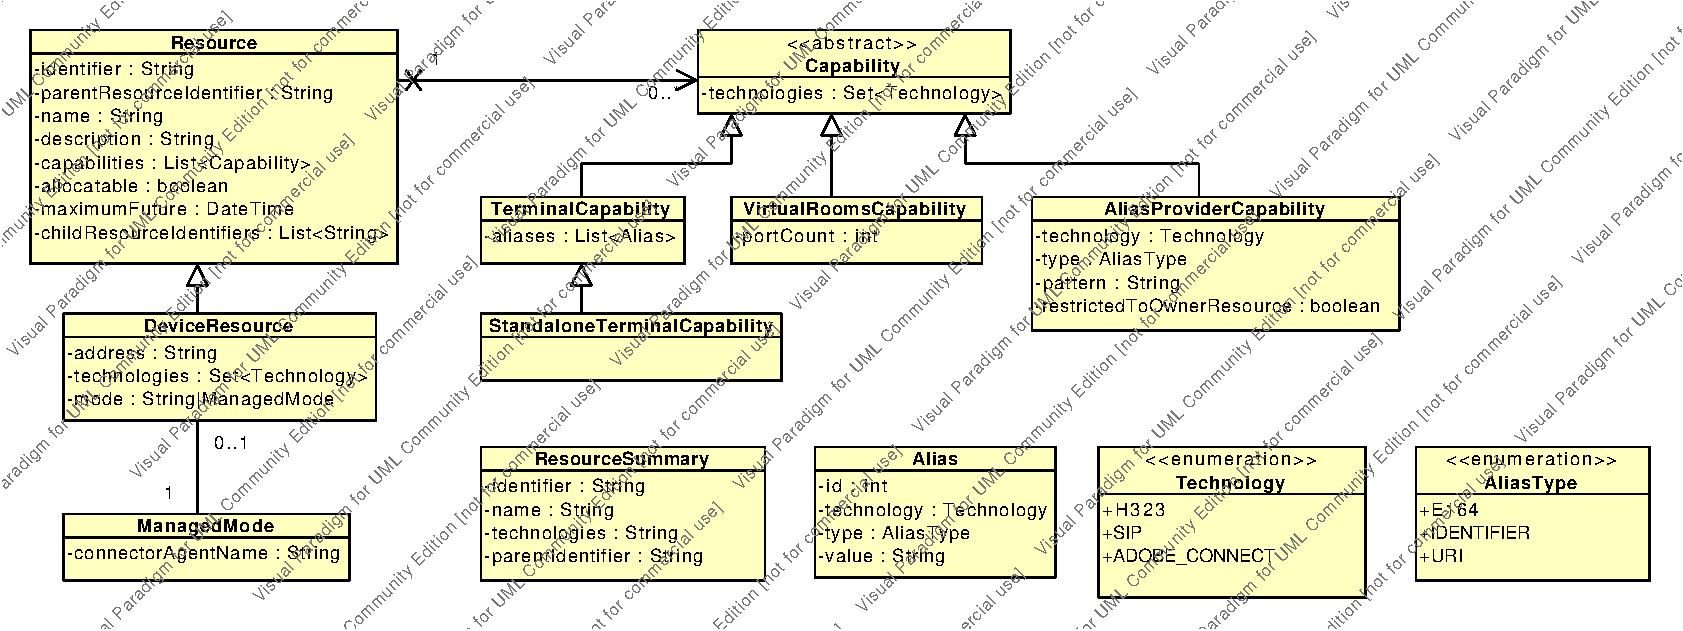
\includegraphics[width=\textwidth]{diagrams/cd_resources_api}
\label{fig:cd_resources}
\caption{Class diagram for \gls{g:resource} database in the \gls{g:controller} API}
\end{figure}

A \gls{g:resource} can be created by an instance of \code{Resource} class. Each \gls{g:resource} is identified by an unique \code{identifier} which is generated by the \gls{g:controller} when the \gls{g:resource} is created in the database.
